\chapter{Experiment Data and Analysis}

\section{Overview of The Balloon Experiments}

High altitude balloons have an extensive heritage as platforms for experiments that take place in the upper atmosphere. In this chapter we will examine results from three balloon flight campaigns which carried X-ray spectrometers. The results of the previous chapters will be applied to determine as much information about the causative precipitating electrons as possible, while avoiding over-fitting the available data. The total precipitating flux and energy distribution of the electrons will be the main targets. The experiments on the balloon flights that we use in this chapter were all equipped with NaI scintillator detectors, and the analysis will be framed around the data that can be obtained from them. There will be questions that can be answered using detectors of a different design, particularly, those sensitive to the angular distribution of the incoming photons. These will be discussed at the end and left for future work. 

The balloon flights used in this analysis were from the following campaigns.

\begin{center}
\begin{tabular}{ |c|c|c|c| } 
\hline
Project Name & Location & Active & Primary Reference \\
\hline
$\text{ABOVE}^2$ & Saskatoon, Saskatchewan & Summer 2016 & None Current\\
\hline
BARREL & Antarctica & 2013-2014 & \citet{Millan2014}\\
\hline
EPEX & Fort MacMurray, Alberta & Summer 2018 & None Current\\
\hline
\end{tabular}
\end{center}

The campaigns each consisted of a number of flights. Each had a somewhat different scientific target, which will be discussed in their analysis sections, however, all of them carried NaI scintillation detectors of a similar design, which we can use with the results from the previous two chapters. We will begin with a discussion of the detector design and operating principles. 

\section{Detector Design}

The sodium iodide scintillation detector carried by flights on all three balloon campaigns was designed by Dr. Michael McCarthy at the University of Washington, Seattle campus. The instrument design has a heritage extending back to~\citet{winckler}. The instrument specifications for the BARREL campaign flights follow, reproduced from~\citet{Millan2014}. 

\begin{center}
\begin{tabular}{ |c|c|c|c|c| }
\hline
Attribute & Value & Comments \\
\hline
Mass & 2.8 Kg & includes insulation and harness \\
Energy Range & 20 keV to 10 MeV & \\
Electronics Resolution & 2.4 keV / channel & reduced by binning \\
System Resolution & 7 percent at 662 keV & \\
Effective Area & 16$\text{ cm}^2$ at 1 MeV & \\
Dead time Per Event & 52 $\mu\text{s}$ & \\
Operating Temperature & -10 to 40 deg C & efficiency decreases below 15 deg C \\
Voltage Requirement & +/- 5 V DC & \\
Current Requirement & 40 mA +, 10 mA - & depends on count rate\\
\hline
\end{tabular}
\end{center}

Simulations completed with GEANT3 (the predecessor to GEANT4) indicate that the detector behaves as essentially uncollimated, though the view through the atmosphere results in it having a field of view of approximately 60 degrees~\citet{Millan2014}. 

A picture of the detector as flown on the $\text{ABOVE}^2$ campaign is shown in Figure~\ref{detector_picture}. The unit is cylindrical, standing on a plexiglass mount and standing approximately 30 cm tall. The cylinder includes the NaI scintillation crystal, photomultiplier tube, and optical coupling. X-rays deposit their energy in the NaI crystal, and a fraction of the resulting light pulse is converted to a voltage pulse by the photomultiplier tube~\citet{Millan2014}. This voltage pulse is then converted to a digital value proportional to the deposited energy by the DPU and output on a serial port for processing and storage by the rest of the flight system. The disconnected wire harnesses visible in Figure~\ref{detector_picture} connect the detector to the various support hardware included with the flight system. Temperature sensors and heaters were used to maintain the detector temperature at 15 deg. C during the flight. Power was provided by an array of lithium-ion rechargeable batteries, which are contained in the rectangular foam box behind the detector in Figure~\ref{detector_picture}.

\begin{figure}[p]
    \centering
    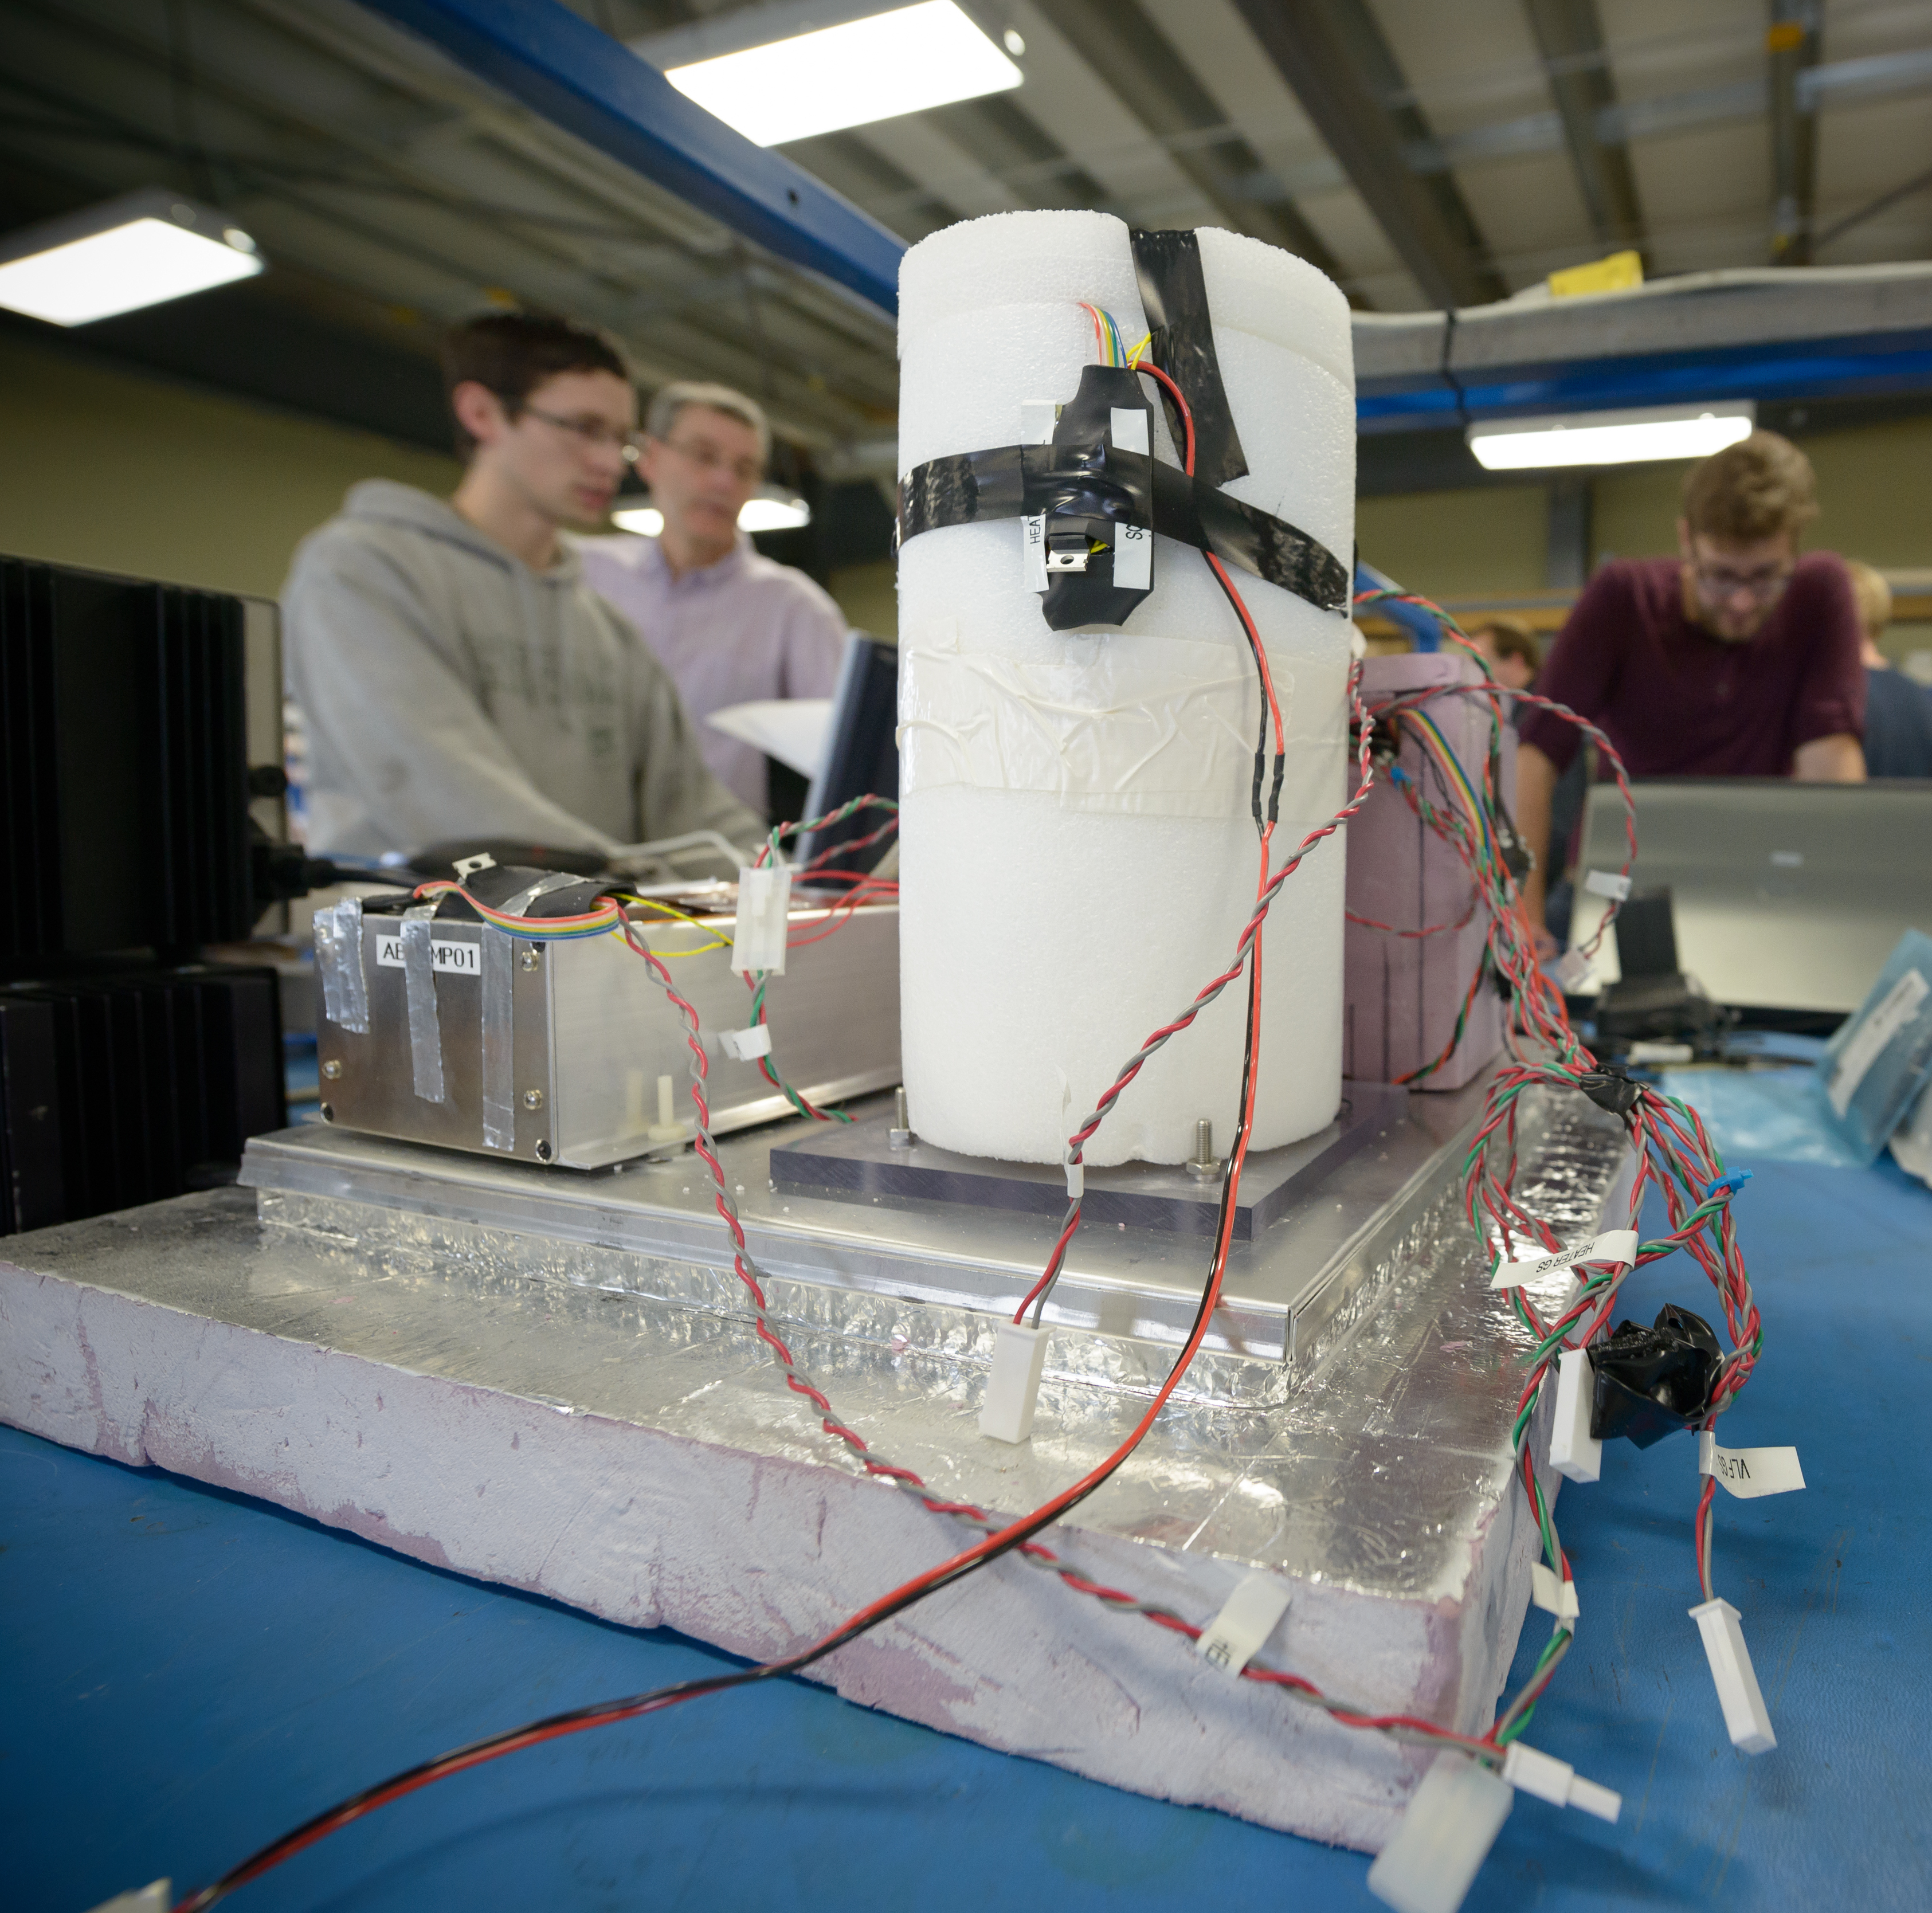
\includegraphics[width=1.0\textwidth]{figures/chapter_5/detector_picture/detector_picture.jpg}
    \caption{X-ray spectrometer (white cylinder) encased in insulation foam and installed with flight systems in balloon payload. The DPU (digital processing unit) is contained in the metal rectangular enclosure on the left. The lead collimator assembly is hidden under the white styrofoam insulation.}
    \label{detector_picture}
\end{figure}

The detector sends measurements to a serial port as digital data. The outputs, reproduced from~\citet{Millan2014}, follow.

\begin{center}
\begin{tabular}{ |c|c|c|c|c| }
\hline
Product & Cadence & Energy Range (keV) & No. of Energy Channels \\
\hline
Rate Counters & 4 & - & - \\
Fast Spectra & 0.05 & 20-1500 & 4 \\
Medium Spectra & 4 & 100-4000 & 48 \\
Slow Spectra & 32 & 20-10000 & 256 \\
\hline
\end{tabular}
\end{center}

For the EPEX and $\text{ABOVE}^2$ campaigns, the instruments were designed to be recovered, and the data were recorded to onboard storage, with some telemetered results as a backup. For the BARREL campaign, the logistics involved in recovering all the payloads are difficult. While a subset were recovered, most were not, and the data were telemetered using an iridium satellite modem. For these flights, the analysis uses the data products published at NASA CDAWEB. The primary citation for this data set is~\citet{Millan2014}.

The functional layout of the detector is shown in the block diagram of Figure~\ref{detector_block_diagram}, which is reproduced from~\citet{Millan2014}.

\begin{figure}[p]
    \centering
    \includegraphics[width=1.0\textwidth]{figures/chapter_5/detector_block_diagram/detector_block_diagram}
    \caption{Block diagram of X-ray scintillation detector system}
    \label{detector_block_diagram}
\end{figure}

\newpage

\section{The $\text{ABOVE}^2$ Campaign}


The $\text{ABOVE}^2$ balloon campaign was flown during the Summer of 2016. There were three flights, each using zero-pressure balloons manufactured by Near-Space Corporation, and designed for a float altitude of greater than 33 kilometers. The first flight was done to validate the operational aspects of the balloon system and telemetry. Flights 2 and 3 were equipped with the X-ray spectrometer. Flight 2 did not see any X-rays besides the expected background, however flight 3 observed a precipitation event that lasted several minutes. Unfortunately, flight 3 had to be flown using the X-ray spectrometer recovered from flight 2, due to an error during installation which damaged the flight 3 spectrometer. This normally wouldn't be a problem, except that the landing under parachute at the end of flight 2 created a shock which was later found to have damaged the crystal, and potentially the optical coupling between the crystal and photomultiplier tube. The effect of these defects is difficult to fully quantify post-flight, except to note that the energy calibration of the detector certainly changes. Further, damage to the optical coupling between the crystal and the photomultiplier tube will result in fewer photons created in the crystal reaching the photomultiplier tube, which will effectively reduce the detector sensitivity. These effects degrade the accuracy and precision of the results from the third $\text{ABOVE}^2$ flight, an effect which will be amplified during the application of the inversion techniques discussed in Chapter~4. Despite these problems, there is still value in examining the data set. The location, timing, and relative amplitudes of the X-ray event are intact, and a comparison between the observed X-ray flux and measurements from a nearby VLF (very low frequency) receiver site shows a strong, though not unexpected, correlation. Figure~\ref{abv2_launch} shows $\text{ABOVE}^2$ science flight 2 being prepared for launch. 

\begin{figure}[p]
    \centering
    \includegraphics[width=1.0\textwidth]{figures/chapter_5/abv2_launch/abv2_launch}
    \caption{$\text{ABOVE}^2$ balloon being filled and prepared for launch in Saskatoon, Saskatchewan, August 2016. The payload and flight train are laid out on the ground, extending approximately 10 meters to the right. Image credit: Joel Kesler / RMD Engineering.}
    \label{abv2_launch}
\end{figure}

\begin{figure}[p]
    \centering
    \includegraphics[width=1.0\textwidth]{figures/chapter_5/abv2_counts/abv2_counts2.pdf}
    \caption{$\text{ABOVE}^2$ X-ray detector counts per second, summed across all energy channels, as a function of time since power-on of the system.}
    \label{abv2_counts}
\end{figure}

Figure~\ref{abv2_counts} shows the total counts recorded by the X-ray spectrometer on science flight 2 as a function of time. After power-on and while the detector is still on the ground, the total counts are roughly constant. Once the balloon is launched (approximately 180 minutes since power on), the detector is removed from naturally occurring radioactive materials in the ground, and the count rate decreases. As altitude increases during the ascent, the count rate starts to increase, because the atmosphere, which acts as a shield from natural radiation from space, begins to decrease in density. After the balloon reaches equilibrium with the atmosphere, the count rates are again roughly constant. On descent, the reverse of this process occurs. The precipitation event observed by science flight 2 happens at approximately 400 minutes from power-on, and lasts for approximately 20 minutes. This is a very weak event.

A background-subtracted spectrum for the precipitation event is shown in Figure~\ref{abv2_hist}. The background was subtracted by taking an average spectrum of the recorded data before the event happened. Above approximately 200 keV, the background subtracted spectrum becomes ragged because it is not distinguishable from the background spectrum. Second-order Tikhonov regularization with preconditioning was applied to the background subtracted spectrum from 30 keV to 200 keV to obtain a model spectrum using a regularization parameter of $\alpha = 10^5$, determined using cross-validation. The solution is shown in Figure~\ref{abv2_tk_inv}. There is not much structure in the solution, due to the application of a high degree of regularization ($\alpha = 10^5$).

Figure~\ref{abv2_tk_inv}} shows that the best model generated by regularization fails to describe the data in the low energy region. The high value of $\alpha $ found through cross-validation reflects this fact and reduces the amount of detail in the model accordingly. The model spectrum has an average energy of approximately 150 to 200 keV. The width of the distribution is not able to be effectively determined for this data set owing to the high value of $\alpha$. 

The regularized solution fails to qualitatively describe the measured X-ray spectrum. An attempt to fit exponential and mono-energetic spectra to the event have the same problem. Fitting to the available data in high energy ranges (more than 150 keV) results in model spectra that ``overshoot'' the measured data in lower energy ranges. This indicates a problem with the data rather than the fitting procedures.

It is believed that the detector was damaged on a previous flight, resulting in measured data that cannot be described by any model. 

\begin{figure}[p]
    \centering
    \includegraphics[width=1.0\textwidth]{figures/chapter_5/abv2_hist/abv2_hist}
    \caption{Background-subtracted X-ray energy spectrum of the precipitation event observed by $\text{ABOVE}^2$ science flight 2. The integration time is 900 seconds, and the bin width is 1 keV.}
    \label{abv2_hist}
\end{figure}

\begin{figure}[p]
    \centering
    \includegraphics[width=1.0\textwidth]{figures/chapter_5/abv2_tk_inv/abv2_fit_problem_4}
    \caption{Application of Tikhonov regularization to the background-subtracted precipitation event measured by $\text{ABOVE}^2$ science flight 2. The algorithm applied is as described in Chapter 4. Second-order regularization with left and right preconditioning is applied together with a positivity constraint to generate the solution.}
    \label{abv2_tk_inv}
\end{figure}

\newpage
\section{The EPEX Campaign}

The EPEX balloon campaign was flown in August, 2018 at Fort McMurray, Alberta, Canada. The campaign had similarities to the $\text{ABOVE}^2$ flights, but had the primary goal of testing a new generation of X-ray detector which used a coded-aperture approach to generate images of the X-ray distributions caused by electron precipitation. My role in the EPEX project consisted of the following:

\begin{itemize}
\item Design and construction of the flight train and mechanical harnessing for the payload.
\item Design and construction of the thermal and electrical support systems for the X-ray instruments.	
\item Implementation of a dual-mode radio tracking and telemetry system consisting of both VLOS (visual line of sight) and BVLOS (beyond visual line of sight) satellite and point to point radio modems.
\item Instrument testing after integration to the payload
\end{itemize}

The analysis of data from the new detector is outside the scope of this thesis. Some of the EPEX flights carried an instrument which was functionally identical to the one flown on $\text{ABOVE}^2$. One of the flights which carried this instrument observed an intense precipitation event while it was at altitude. The event is shown in spectrogram form in Figure~\ref{epex_event_spectrogram}. Immediately apparent is the temporal structure and how it differs from the $\text{ABOVE}^2$ event. This event started at a sharply defined time (6:40 UT, see Figure~\ref{epex_event_spectrogram}) and quickly reached its peak before decaying. The fact that the intensity was so high makes this a good target for the application of the inversion techniques used in Chapter~4. 

\begin{figure}[p]
    \centering
    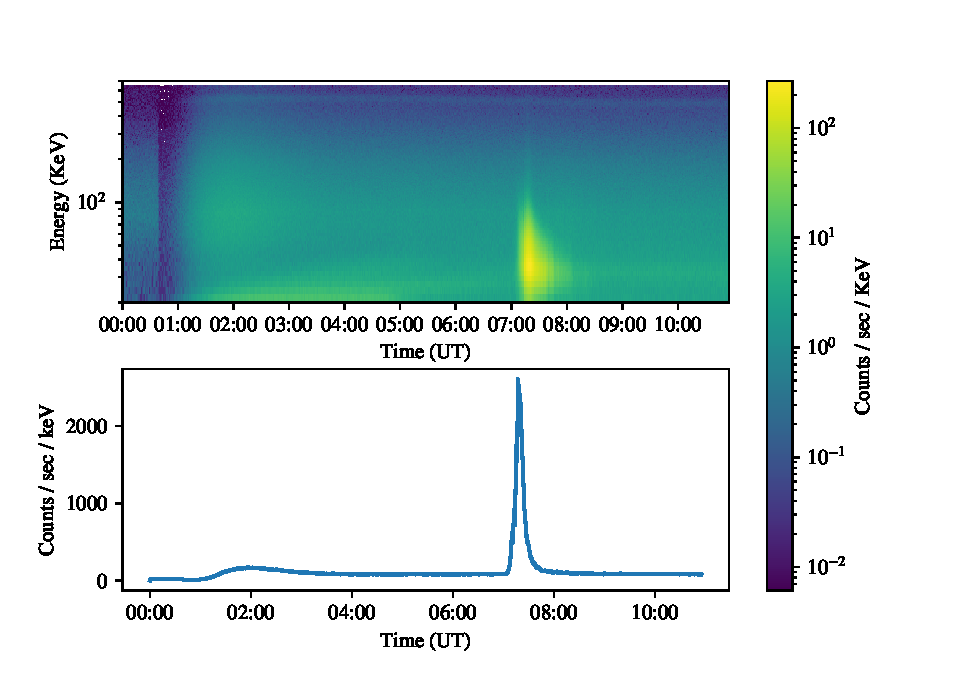
\includegraphics[width=1.0\textwidth]{figures/chapter_5/epex_spectrogram/epex_spectrogram__with_cps_cbar-2}
    \caption{EPEX X-ray spectrometer data in spectrogram form. The precipitation event was observed at 07:00 UTC. The total counts per second are shown below the spectrogram as a function of time.}
    \label{epex_event_spectrogram}
\end{figure}

A background-subtracted spectrum of the precipitation event is shown, along with the reconstruction using the techniques of Chapter 4, in Figure~\ref{epex_fit_comparison}. The retrieved precipitating electron spectrum is shown in Figure~\ref{epex_tk_inv}. It was generated using second-order Tikhonov regularization with left and right diagonal preconditioning and a positivity constraint. The X-ray spectrum data from 70 to 500 keV were fit. The retrieved electron spectrum has a very mono-energetic structure at approximately 80 keV. The model agrees well with the data, unlike the result from the $\text{ABOVE}^2$ event, because this detector was flown in a refurbished and undamaged state. The total precipitating electron flux is estimated by the model as $4.8\times 10^8$ electrons $\text{cm}^2$ / second. This was a very bright event which was well-defined in time and energy. The low value of $\alpha = 3.5\times10^3$ (compared to the $\text{ABOVE}^2$ event) suggested by cross-validation indicates that a good fit to the data was found by the reconstruction algorithms without requiring intense reconditioning of the problem. This is consistent with the fact that this bright event has a very high signal to noise ratio in the background subtracted data. This event can serve as an example of the usefulness of the regularization techniques in analyzing X-ray data. The regularized model in Figure~\ref{epex_fit_comparison} shows better agreement with the data than either the best exponential or monoenergetic fits. The reduced $\chi ^2$ statistics for the monoenergetic and exponential fits are 0.53 and 58.0, respectively. The reduced $\chi ^2$ for the regularized model is 0.75. This indicates that the exponential fit is a bad description of the X-ray data set for this event. The monoenergetic fit is better, but the regularized solution is best, having a reduced $\chi ^2$ statistic closest to 1.0. The strength of the regularization methods, combined with cross-validation, is that, with mild assumptions, we can a model-independent characteristic energy and width of the electron distribution. 

\begin{figure}[p]
    \centering
    \includegraphics[width=1.0\textwidth]{figures/chapter_5/epex_fit_comparison/epex_fit_comparison2.pdf}
    \caption{Background-subtracted X-ray event measured by the EPEX spectrometer. The model fit using Tikhonov regularization is shown overlaid.}
    \label{epex_fit_comparison}
\end{figure}

\begin{figure}[p]
    \centering
    \includegraphics[width=1.0\textwidth]{figures/chapter_5/epex_tk_inv/epex_tk_inv2.pdf}
    \caption{Precipitating electron spectrum retrieved from EPEX X-ray data using the techniques of Chapter 4. The required value for $\alpha$ is low and well-defined through cross-validation.}
    \label{epex_tk_inv}
\end{figure}

\section{The BARREL Campaign}

I examine one flight from the NASA BARREL balloon campaign, which occurred during 2014. This flight was launched with an X-ray spectrometer similar to those flown on the EPEX and  $\text{ABOVE}^2$ campaigns, and recorded an electron precipitation event while magnetically local to an orbiting spacecraft (Van Allen Probe B), which provides conjugate measurements of energetic electrons via the MAGEIS instrument. This flight was analyzed by~\citet{Halford2015}, who determined that the precipitation event occurred in the aftermath of an ICME (interplanetary coronal mass ejection) shock. Since the BARREL balloon was airborne and recoding data while the spacecraft was on the same approximate L-shell, \citet{Halford2015} could complete an ``end-to-end'' study of the recorded precipitation event, from creation, to detection by an RBSP spacecraft, to the precipitation in the atmosphere and resulting creation of X-ray radiation detected by the balloon. We will analyze the event measured by the balloon in this section.

A spectrogram of the event observed by~\citet{Halford2015} is shown in Figure~\ref{barrel_spectrogram}. This is a very low intensity event, but it occurs over a time period of tens of minutes. We will use an average spectrum taken over the event time range. The background-subtracted spectrum of the event, and the best-fit model spectrum is shown in Figure~\ref{barrel_fit_comparison.}. Finally, the retrieved electron spectrum is shown in Figure~\ref{barrel_tk_inv}. The retrieved electron spectrum has two main components, a distribution at around 250 keV, and a smaller high energy component at around 600 to 700 keV. The significance of the high energy component is not clear, since the X-ray spectrum has a noise floor which begins at approximately 200 keV. 

\begin{figure}[p]
    \centering
    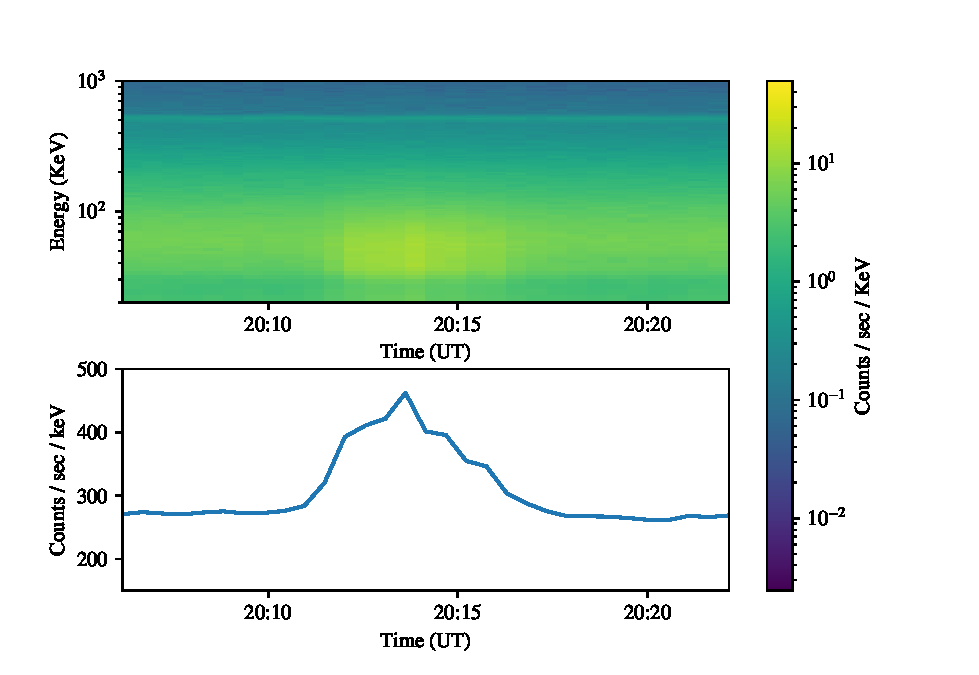
\includegraphics[width=1.0\textwidth]{figures/chapter_5/barrel_spectrogram/barrel_spectrogram}
    \caption{Spectrogram and raw count rates of the event measured by BARREL and studied by~\citet{Halford2015}.}
    \label{barrel_spectrogram}
\end{figure}

\begin{figure}[p]
    \centering
    \includegraphics[width=1.0\textwidth]{figures/chapter_5/barrel_fit_comparison/barrel_fit_comparison}
    \caption{Background-subtracted X-ray event measured by the BARREL spectrometer. The model fit using Tikhonov regularization is shown overlaid.}
    \label{barrel_fit_comparison}
\end{figure}

\begin{figure}[p]
    \centering
    \includegraphics[width=1.0\textwidth]{figures/chapter_5/barrel_tk_inv/barrel_tk_inv}
    \caption{Precipitating electron spectrum retrieved from BARREL X-ray data using the tfechniques of Chapter 4. The required value for $\alpha$ is approximately $5\times10^2$.}
    \label{barrel_tk_inv_2}
\end{figure}

\subsection{Energy Selective Scattering}

As a validation of the inversion method, the electron spectrum can be compared with in-situ measurements of the corresponding electron flux measured by the satellite in the magnetosphere. The in-situ data provides a limit on the precipitating electron flux, which is the product of the available flux and the scattering efficiency. A subset of the flux measured by the satellite will precipitate into the atmosphere.  

Spacecraft measurements of energetic electrons do not generally resolve the population within the loss cone.  We show that the techniques developed in Chapter~4 can be applied to infer this energy range from balloon measurements, by building on an analysis published by~\citet{Halford2015}. \cite{Halford2015} reported on an energetic electron precipitation event that happened while one of the Van Allen Probe B was at a similar L-value and close in MLT with a BARREL balloon 2L that measured the resulting X-ray spectrum. Their analysis provides an end-to-end picture that describes the scattering processes which drove the event, and the measurable impact it made on the atmosphere.  

The Van Allen Probes are a pair of orbiting spacecraft which carry instruments to understand electron acceleration in the radiation belts. The Magnetic Electron Ion Spectrometer (MAGEIS) instruments are magnetic spectrometers that provide in-situ measurements of the energies, angular distributions, and differential fluxes of electrons in the radiation belts~\cite{Blake2013,Spence2014}. There are four magnetic spectrometers on each spacecraft, each designed for a specific energy range. Electrons enter each instrument through a collimator and are deflected to a pixelated detector surface by a uniform magnetic field. We will use the pitch angle resolved, background-subtracted differential energy fluxes provided by the Energetic Particle, Composition, and Thermal Plasma (RBSP-ECT) investigation~\cite{Spence2013}.

A key assumption that must be made in the analysis of the precipitation event from~\cite{Halford2015} is that the available MAGEIS data in the lowest (approx. 8 degree)  pitch angle bin represents the energy distribution of electrons that are scattered into the loss cone. This is because MAGEIS does not resolve fluxes within the loss cone. The assumption is that the electron spectrum in the loss cone is the same as the electron spectrum in the lowest pitch angle bin, except that it has undergone a scattering process which selects for a range of electron energies. but leaves the rest of the spectrum unaltered. ~\cite{Thorne2010} uses quasi-linear theory and satellite data to show that chorus waves lead to rapid pitch angle scattering over a narrow pitch angle range near the loss cone for electrons from 100 eV to a few keV. 

 \cite{Halford2015} apply exponential and mono energetic fits to the measured X-ray data, and also compared with the energy spectra observed near the loss cone from Van-Allen Probe B MagEIS data which was at a similar L-value and close in MLT to BARREL payload 2L (see Figure 4 in \cite{Halford2015}). The best fit to the observed X-ray spectra was found when using the observed energy spectra from Van Allen Probe B. The agreement reveals that the measured event does contain enough information to distinguish between electron beams with zero width (mono-energetic), and beams which extend to the highest modelled energy (exponential). We use this event as a test of the regularization method to see how much more information about the scattered electron spectrum it can extract. In particular, under the assumption that the scattering processes responsible for the observed precipitation select an energy range from the magnetically conjugate Van-Allen Probe measured electron spectrum, we evaluate if that energy range can be determined from the X-ray data. 

The comparison of mono-energetic and exponential fits to the balloon X-ray spectrum done by~\cite{Halford2015} is reproduced in Figure~\ref{barrel_electron_fit_comparison}. We apply the constrained second-order regularization technique to obtain a model electron spectrum. The X-ray spectrum predicted to result from this retrieved spectrum is plotted with the measured X-ray data, and shows closer agreement with the BARREL spectrum than the best fits that can be produced by assuming the mono-energetic or exponential forms. 

\begin{figure}[p]
    \centering
    \includegraphics[width=1.0\textwidth]{figures/chapter_5/barrel_electron_fit_comparison/barrel_fit_comparison_2}
    \caption{Mono-energetic and exponential fits to the BARREL event from ~\cite{Halford2015}, with the fit obtained by applying the techniques developed in Chapter~4 (preconditioned, constrained second-order Tikhonov regularization using cross-validation). The total electron flux for the regularized model is found to be $1.6 \times 10^6 \mbox{electrons}/\mbox{cm}^2/\mbox{sec}$.}
    \label{barrel_electron_fit_comparison}
\end{figure}

Data from the RBSP MAGEIS instrument used in the analysis of the ~\cite{Halford2015} event is shown in Figure~\ref{mageis_spectrum}. Under the assumption of strong scattering, with a full loss cone. The topside electron flux from a spacecraft in magnetic conjunction with a given location on Earth is given as $F\approx (B_{i}/B_{top}) J_{top} \Delta \Omega$ ~\citep{kasahara2018}. $B_{i}$ and $B_{top}$ are the magnetic field strengths at the precipitation point and spacecraft, and $J_{top}$ is the electron flux at the spacecraft. $\Delta \Omega$ is the width of the loss cone at the spacecraft. 

This estimate requires the assumption that the electrons measured in the lowest pitch angle bin of the MAGEIS data (approximately 8 degrees) represent the energy spectrum of electrons in the loss cone. The radio of solid angles subtended by 8 degrees and 2.5 degrees is $10.22$. The ratio of magnetic field strengths at the MAGEIS instrument and at the balloon is approximately $150 \text{nT}/55000{nT} = 366.6$. Using this, the expected precipitating electron spectrum based on the MAGEIS data is shown in Figure~\ref{mageis_spectrum}. The inferred precipitating electron spectrum based on the regularized solution from the balloon data is shown in the same units. 

\begin{figure}[p]
    \centering
    \includegraphics[width=1.0\textwidth]{figures/chapter_5/mageis_spectrum/mageis_spectrum_2}
    \caption{Expected precipitating electron spectrum as measured by RBSP-B MAGEIS and model spectrum generated from measured balloon data using Tikhonov regularization.}
    \label{mageis_spectrum}
\end{figure}

The precipitating spectrum inferred from the measured balloon data is subset to the spectrum predicted to precipitate from the MAGEIS data. This is an expected result, since the electron population in the loss cone at the spacecraft represents a total available flux which can precipitate, while the balloon spectrum represents the actual population that did precipitate and impact the atmosphere. This supports the value of balloon measurements of precipitating electron spectra. The shape of the energy spectrum obtained from the balloon data is different than the population measured by the MAGEIS instrument on the spacecraft. The determination of this shape using Tikhonov regularization represents additional information which is available in the balloon X-ray data, which is not retrieved when fitting assumed forms for the precipitating electron spectrum. The information carried by the shape of the precipitating spectrum also represents information about the scattering processes responsible for the precipitation, since they are energy dependent. 






